\documentclass{report} 
\usepackage{amsmath}
\usepackage{amssymb}
\usepackage[a4paper]{geometry}
\usepackage{graphicx}
\usepackage{xcolor}
\usepackage{multirow}
\usepackage{bm}

% Personnalised commands

\newcommand{\eg}{\mathrm{e.g.}}
\newcommand{\rhs}{\mathrm{rhs}}
\newcommand{\kB}{k_\mathrm{B}}
\newcommand{\mH}{m_\mathrm{H}}
\newcommand{\mel}{m_\mathrm{e^-}}
\newcommand{\nelin}{n_\mathrm{e^-, \, in}}
\newcommand{\rhat}{\hat{\bm{r}}}
\newcommand{\ro}{\bm{r}_0}
\newcommand{\rv}{\bm{r}}
\newcommand{\xiv}{\bm{\xi}}
\newcommand{\taumax}{\tau^\mathrm{max}}
\newcommand{\Dtau}{\Delta \tau}
\newcommand{\kext}{\kappa^\mathrm{ext}}
\newcommand{\cosi}{\cos{i}}
\newcommand{\sini}{\sin{i}}
\newcommand{\cosdi}{\cos^2{i}}
\newcommand{\sindi}{\sin^2{i}}
\newcommand{\tandTheta}{\tan^2{\Theta}}
\newcommand{\Rstar}{R_\mathrm{\star}}
\newcommand{\Tstar}{T_\mathrm{\star}}
\newcommand{\loggstar}{\log{(g_\mathrm{\star})}}
\newcommand{\mhstar}{[M/H]_\mathrm{\star}}
\newcommand{\Mstar}{M_\mathrm{\star}}
\newcommand{\Jnustar}{J_\nu^\mathrm{\star}}
\newcommand{\mustar}{\mu_\mathrm{\star}}
\newcommand{\taunustar}{\tau_\nu^\mathrm{\star}}
\newcommand{\Inustar}{I_\nu^\mathrm{\star}}
\newcommand{\nuo}{\nu_{0}}
\newcommand{\Bnu}{B_\nu}
\newcommand{\Snu}{S_\nu}
\newcommand{\knuabs}{\kappa_{\nu}^\mathrm{abs}}
\newcommand{\knusca}{\kappa_{\nu}^\mathrm{sca}}
\newcommand{\knuext}{\kappa_{\nu}^\mathrm{ext}}
\newcommand{\Rind}{R_\mathrm{in, \, d}}
\newcommand{\Routd}{R_\mathrm{out, \, d}}
\newcommand{\nd}{n_\mathrm{d}}
\newcommand{\nind}{n_\mathrm{in, \, d}}
\newcommand{\alphad}{\alpha_\mathrm{d}}
\newcommand{\betad}{\beta_\mathrm{d}}
\newcommand{\gammad}{\gamma_\mathrm{d}}
\newcommand{\Hd}{H_\mathrm{d}}
\newcommand{\Hind}{H_\mathrm{in, \, d}}
\newcommand{\hind}{h_\mathrm{in, \, d}}
\newcommand{\Td}{T_\mathrm{d}}
\newcommand{\Tind}{T_\mathrm{in, \, d}}
\newcommand{\Cnuextd}{C_{\nu, \, \mathrm{d}}^\mathrm{ext}}
\newcommand{\Cnuoextd}{C_{\nu_0, \, \mathrm{d}}^\mathrm{ext}}
\newcommand{\taunuod}{\tau_{\nu_0, \, \mathrm{d}}}
\newcommand{\knuextd}{\kappa_{\nu, \, \mathrm{d}}^\mathrm{ext}}
\newcommand{\knuoextd}{\kappa_{\nu_0, \, \mathrm{d}}^\mathrm{ext}}
\newcommand{\Qnuextd}{Q_{\nu, \, \mathrm{d}}^\mathrm{ext}}
\newcommand{\amin}{a_\mathrm{min}}
\newcommand{\amax}{a_\mathrm{max}}
\newcommand{\gbff}{\bar{g}_\nu^\mathrm{bf + ff}}
\newcommand{\Routg}{R_\mathrm{out, \, g}}
\newcommand{\nel}{n_\mathrm{e^-}}
\newcommand{\xion}{x_{ion}}
\newcommand{\Eion}{E_\mathrm{ion}}
\newcommand{\nH}{n_\mathrm{H}}
\newcommand{\nHp}{n_\mathrm{H^+}}
\newcommand{\ngas}{n_\mathrm{g}}
\newcommand{\ning}{n_\mathrm{in, \, g}}
\newcommand{\alphag}{\alpha_\mathrm{g}}
\newcommand{\betag}{\beta_\mathrm{g}}
\newcommand{\gammag}{\gamma_\mathrm{g}}
\newcommand{\Hg}{H_\mathrm{g}}
\newcommand{\Tg}{T_\mathrm{g}}
\newcommand{\Ting}{T_\mathrm{in, \, g}}
\newcommand{\knuabsg}{\kappa_{\nu, \, \mathrm{g}}^\mathrm{abs}}
\newcommand{\knuscag}{\kappa_{\nu, \, \mathrm{g}}^\mathrm{sca}}
\newcommand{\knuextg}{\kappa_{\nu, \, \mathrm{g}}^\mathrm{ext}}
\newcommand{\knuoabsg}{\kappa_{\nu_0, \, \mathrm{g}}^\mathrm{abs}}
\newcommand{\knuoscag}{\kappa_{\nu_0, \, \mathrm{g}}^\mathrm{sca}}
\newcommand{\knuoextg}{\kappa_{\nu_0, \, \mathrm{g}}^\mathrm{ext}}
\newcommand{\taunug}{\tau_{\nu, \, \mathrm{g}}}
\newcommand{\taunuog}{\tau_{\nu_0, \, \mathrm{g}}}
\newcommand{\ulam}{\frac{u_{1,2}}{\lambda}}
\newcommand{\vlam}{\frac{v_{1,2}}{\lambda}}
\newcommand{\xI}{x_\mathrm{I}}
\newcommand{\yI}{y_\mathrm{I}}
\newcommand{\rI}{r_\mathrm{I}}
\newcommand{\thetaI}{\theta_\mathrm{I}}
\newcommand{\aI}{a_\mathrm{I}}
\newcommand{\muI}{\mu_\mathrm{I}}
\newcommand{\nuI}{\nu_\mathrm{I}}
\newcommand{\Nuv}{N_{u, \, v}}
\newcommand\underrel[2]{\mathrel{\mathop{#2}\limits_{#1}}}
\newcommand{\Rin}{R_\mathrm{in}}
\newcommand{\Rout}{R_\mathrm{out}}
\newcommand{\Pcal}{\mathcal{P}}
\newcommand{\Gcal}{\mathcal{G}}
\newcommand{\Dcal}{\mathcal{D}}
\newcommand{\Ocal}{\mathcal{O}}
\newcommand{\Fcal}{\mathcal{F}}
\newcommand{\thetamax}{\theta_\mathrm{max}}
\newcommand{\thetamin}{\theta_\mathrm{min}}
\newcommand{\varphimin}{\varphi_\mathrm{min}}
\newcommand{\varphimax}{\varphi_\mathrm{max}}

\title{Notes on ray-tracing}

\author{J. Perdigon}

\begin{document}

\maketitle

\section{Description of the ray tracing tool} \label{Sect:description_ray_tracing}

\begin{figure*}
  \centering
  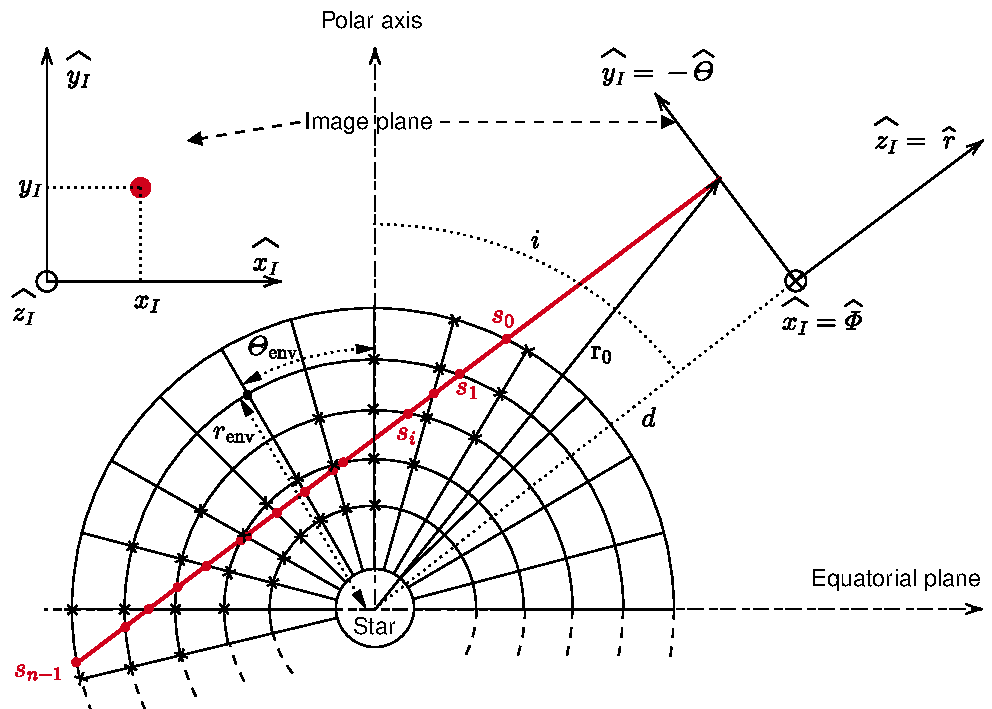
\includegraphics[width=\textwidth]{images/ray_tracing_schematics.pdf}
  \caption{\textcolor{red}{caption}}
  \label{fig:rtSchematic}
\end{figure*}

\begin{figure*}
  \centering
  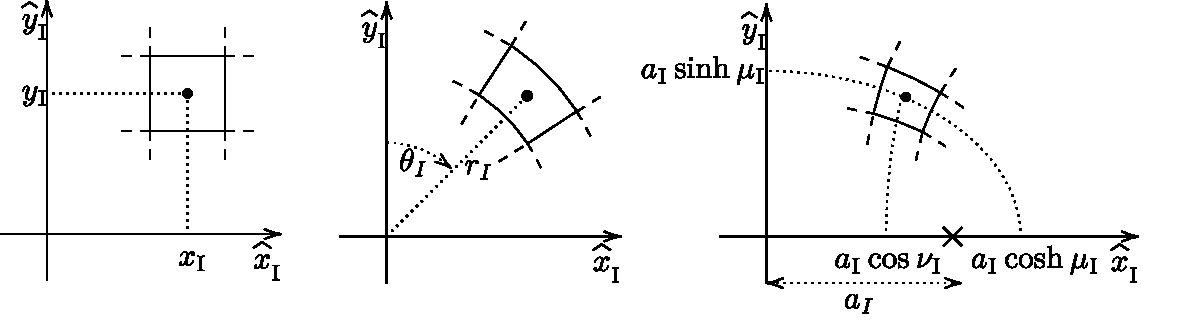
\includegraphics[width=\textwidth]{images/pixel_geometry.pdf}
  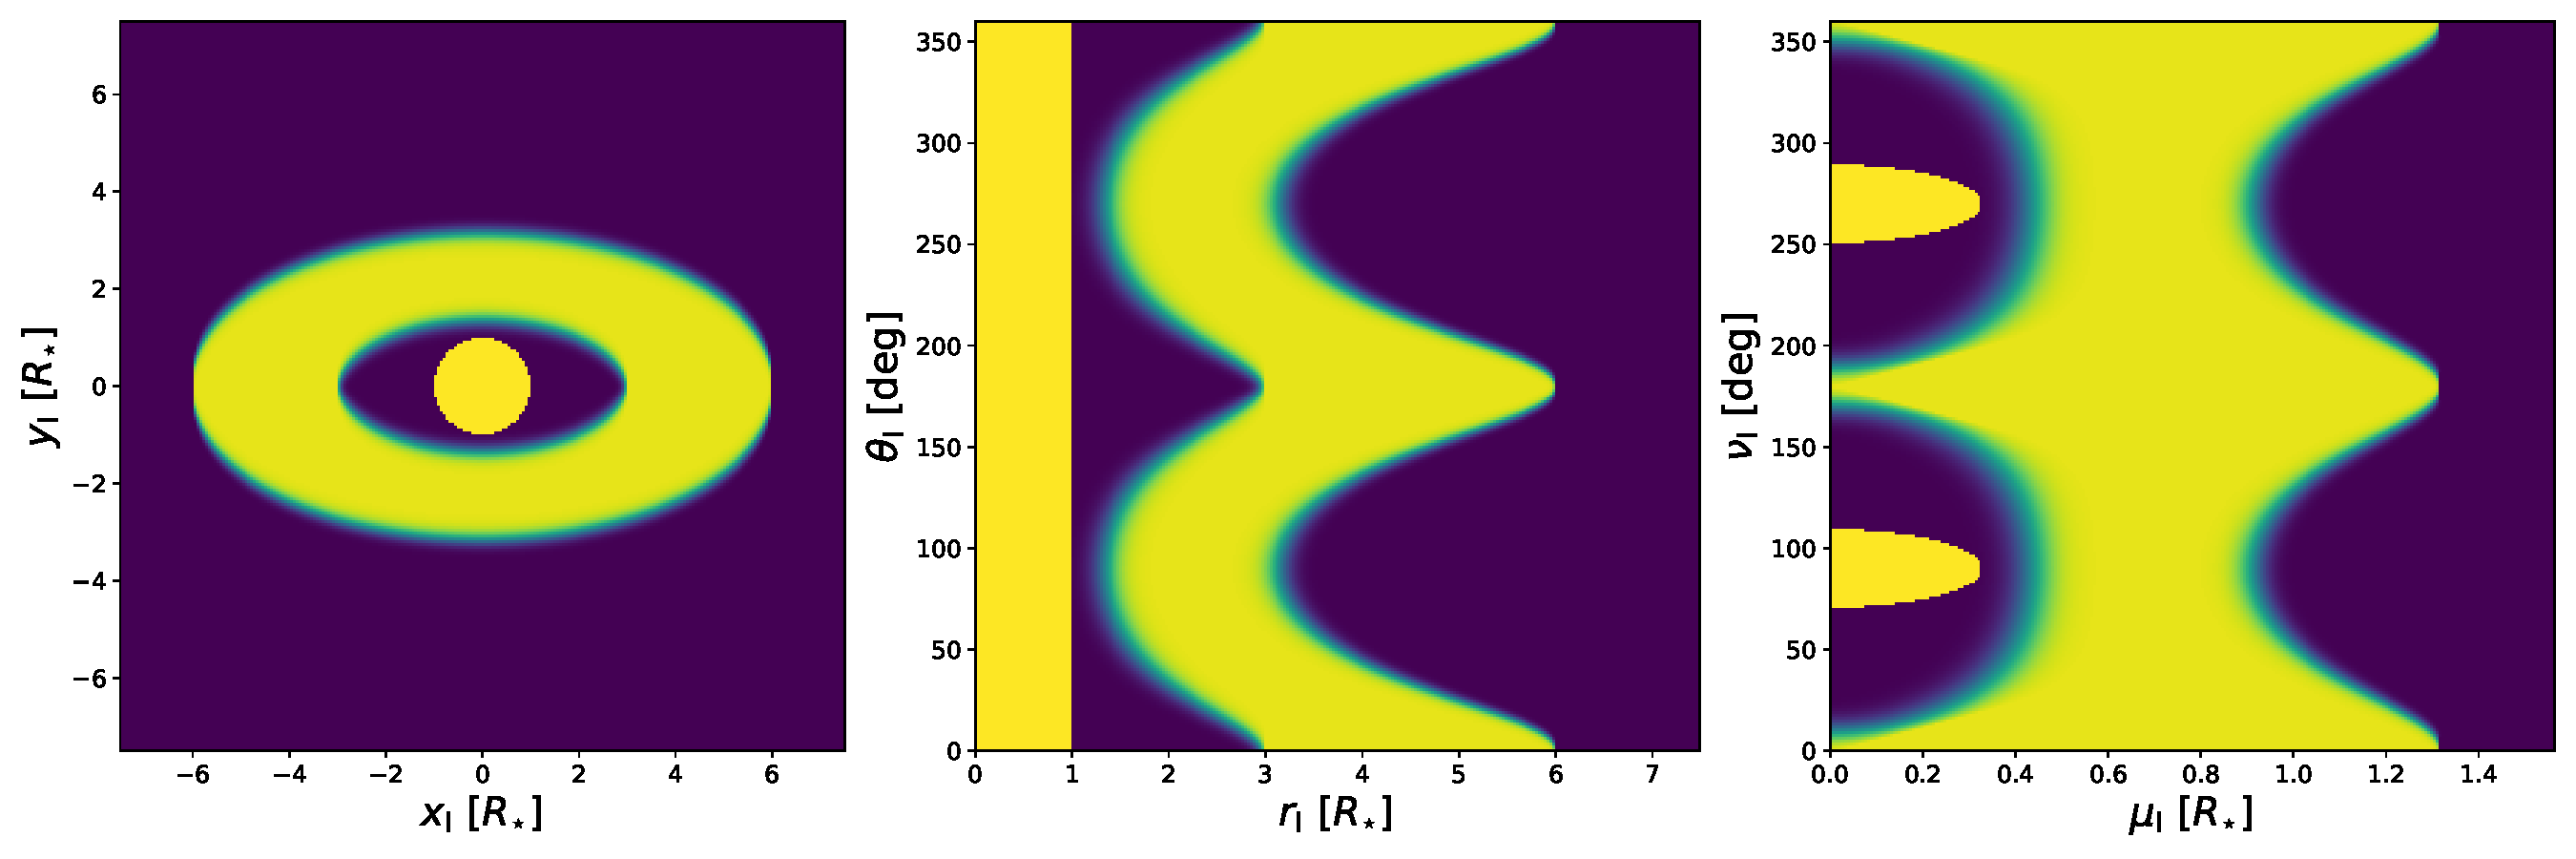
\includegraphics[width=\textwidth]{images/image_geometry.pdf}
  \caption{Example of an image of a dummy disc with $\Rin = 3 \, \Rstar$ and $\Rout = 5 \, \Rstar$, using three different geometries. The top panels display the coordinate system while the bottom ones show the corresponding image. \textit{Left}: Cartesian geometry; the pixel surface $\Delta S$ is $\Delta x \, \Delta y$. \textit{Middle}: Spherical geometry; $\xI = \rI \, \cos{\thetaI}$, $\yI = \rI \, \sin{\thetaI}$ and $\Delta S = \rI \, \Delta \rI \, \Delta \thetaI$, with $\rI \geq 0$ and $\thetaI \in [0, \, 2\pi]$. \textit{Right}: Elliptic geometry; $\xI = \aI \, \cosh{\muI} \, \cos{\nuI}$, $\yI = \aI \, \sinh{\muI} \, \sin{\nuI}$ and $\Delta S = \aI^2 \left( \cosh^2{\muI} \, \cos^2{\nuI} + \sinh^2{\muI} \, \sin^2{\nuI} \right) \Delta \muI \, \Delta \nuI$, with $ \muI \geq 0$ and $\nuI \in [0, \, 2\pi]$. In this example, we set $\aI = \Rin$.}
  \label{fig:geometry}
\end{figure*}

    \begin{table*}
        \caption{List of inputs and outputs of the ray tracing code}
        \label{tab:io_ray_tracing}
        \centering
        \begin{tabular}{c c c c}
            \hline\hline 
            I/O & Description & Symbol & Python data type (shape) \\ 
            \hline
            \multirow{9}{*}{Inputs} 
            & $1^\mathrm{st}$ coordinates of pixels of the image & $\xI$ & 1D-ndarray $(N,)$ \\
            & $2^\mathrm{nd}$ coordinates of pixels of the image & $\yI$ & 1D-ndarray $(N,)$ \\
            & Radial coordinates at the vertices of the circumstellar grid & $r$ & 1D-ndarray $(N_r,)$ \\
            & Angular coordinates at the vertices of the circumstellar grid & $\Theta$ & 1D-ndarray $(N_\Theta,)$ \\
            & Extinction coefficient at the vertices of the circumstellar grid & $\kappa^\mathrm{ext}$ & 3D-ndarray $(N_\lambda, N_r, \, N_\Theta)$ \\
            & Source function at the vertices of the circumstellar grid & $S$ & 3D-ndarray $(N_\lambda, N_r, \, N_\Theta)$ \\
            & Image plane inclination & $i$ & float64 $(1)$ \\
            & Stellar radius & $\Rstar$ & float64 $(1)$ \\
            & Stellar intensity & $\Inustar$ & 1D-ndarray $(N_\lambda,)$ \\
            \hline
            Outputs & Specific intensity map & $I\left(\ro, \, \rhat \right)$ & 2D-ndarray $(N_\lambda, \, N)$ \\
            \hline
        \end{tabular}
        %\tablefoot{\textcolor{red}{caption}}
    \end{table*}
    
    In this section, we present the ray tracing tool\footnote{Publicly available at \textcolor{red}{git link}} we developed in order to compute synthetic images from a given distribution of circumstellar material. The tool was first developed as a complementary module to the discontinuous Galerkin finite element method radiative transfer code from \textcolor{red}{ref}, for computing spectral energy distributions (SEDs hereafter). It was subsequently improved to include more features and developed as standalone package. 

    \subsection{General overview}
    
    First, a given configuration of matter is sampled on the a regular grid around the star. This grid is defined with the spherical coordinate system. We further assume that the distribution of matter is symmetric around the polar axis and symmetric with respect to the equatorial plane. Each vertex of the grid is then only defined by two coordinates $\left(r, \Theta\right)$, with $r$ being the radius and $\Theta$ the co-latitude angle with respect to the polar axis (see $\eg$ the black dot in Fig.~\ref{fig:rtSchematic}).
      
    The image plane is defined with respect to the spherical coordinates system of the grid. It makes an angle $i$ with respect to the polar axis, and $x_I$ and $y_I$ axes coincide with the $\phi$ and $-\Theta$ axes of the spherical coordinates, respectively (see Fig.~\ref{fig:rtSchematic}). 
      
    Each pixel constituting the image is intersected by a ray normal to the image plane (red line in Fig.~\ref{fig:rtSchematic}), along which we want to estimate the specific intensity emitted by the circumstellar material. The intensity at the pixel centre $\ro$, in the direction $\rhat$, omitting the frequency dependence for clarity, can be expressed by the integral form of the radiative transfer equation \textcolor{red}{ref},
    \begin{equation}
      I\left(\ro, \, \rhat \right) = \int \limits_{0}^{\taumax} S\left(\tau\right) \, \exp{\left(- \tau\right)} \, d\tau . \label{eq:intensity}
    \end{equation}
    where $S$ is the source function and $\tau$ is the optical depth along the ray. The optical depth is defined as 
    \begin{equation}
      \tau\left(s\right) = \int \limits_{s_0}^{s} \kext \left(s'\right) \, ds', \label{eq:tau_ray}
    \end{equation}
    with $\kext$ the extinction coefficient and $s$, coordinate along the ray. Eqs.~(\ref{eq:intensity}) and (\ref{eq:tau_ray}) are numerically estimated with the help of the values of $\Snu$ and $\kext$ at the intersections between the ray and the grid (red dots in Fig.~\ref{fig:rtSchematic}). The values at the intersections are linearly interpolated from the closest neighbouring values of the grid (back crosses in Fig.~\ref{fig:rtSchematic}). We give more technical details, in Appendix \ref{sect:desc_ray}, on how the intersections and Eqs.~(\ref{eq:intensity}) and (\ref{eq:tau_ray}) are computed.  
    
    The tool is written in the Python language and encapsulated in a class. The inputs parameters and outputs products are summarised in Table \ref{tab:io_ray_tracing}. In the following, we discuss about some points that might be relevant to the user when using the tool.
    
    To compute an image, the user must input the $\xI$ and $\yI$ positions of each pixel centre. In this way, the tool can compute the intensity map from any given distribution of pixels. In Fig.~\ref{fig:geometry}, we show an example of an image of a dummy disc using 3 different geometries. While the Cartesian geometry has the advantage of allowing the use of the FFT algorithm to compute the physical observables presented in Sect. \textcolor{red}{ref}, it has the disadvantage of not featuring any pixel refinement. The spherical and elliptical geometries however naturally present some degree of pixel refinement, around the centre $(\xI, \, \yI = 0, \, 0)$ and around the two focal points $(\xI, \, \yI = \pm \aI, \, 0)$, respectively. This is a clear numerical advantage, because it means that objects with details around these refinements points will be resolved using a much lower number of pixels in comparison with the Cartesian geometry. The drawback of the the spherical and elliptic geometries is that one cannot use the FFT algorithm to compute the Fourier transform of the image. We discuss the latter point in more details in Sect. \textcolor{red}{ref}.
    
    The user also need to provide the vertices $(r, \, \Theta)$ of circumstellar grid where the extinction coefficient $\kext$ and the source function $\Snu$ are defined. Because in general the values of these quantities span many order of magnitude across several order of magnitude in radius, it is usually necessary to logarithmic sample the radial coordinates of the vertices. For the polar angle $\Theta$, the sampling should be done according the type of object considered. For instance, the user might want to increase the number of points towards the equatorial plane ($\Theta = \pi / 2)$ to correctly sample the density distribution of a circumstellar disc. If polar jets are present, the user might want to also refine the grid around the polar axis $(\Theta = 0)$.
    
  \subsection{Evaluation of the pixel intensity} \label{sect:desc_ray}

   Let us denote by $s$ the path coordinate along the ray, with an increasing value towards the star. The position of a given point on the ray is $\rv\left(s\right) = \ro - s \, \rhat$, with $\ro$, the position of the intersection of the ray with the image plane, and $\rhat$, the unit radial vector normal to the image plane.
   
   In practice, we only know the values of $S$ and $\kext$ at the intersections of the ray with the grid (red dots in Fig.~\ref{fig:rtSchematic}). We then need to assume a specific form for these quantities along each portion between two consecutive intersections. The integral in Eq.~(\ref{eq:intensity}) can be split as
  \begin{equation}
      I\left(\ro, \, \rhat \right) = \sum \limits_{i=0}^{n-2} \int \limits_{\tau\left(s_i\right)}^{\tau\left(s_{i+1}\right)} S\left(\tau\right) \, \exp{\left(- \tau\right)} \, d\tau.
  \end{equation}
  Performing the variable change $t = \tau - \tau(s_i)$,
  \begin{equation}
      I\left(\ro, \, \rhat \right) = \sum \limits_{i=0}^{n-2} \exp{\left(- \tau\left(s_i\right)\right)} \int \limits_{0}^{\Dtau_i} S\left(t\right) \, \exp{\left(- t \right)} \, dt, \label{eq:intensity_2}
  \end{equation}
  with $\Dtau_i = \tau\left( s_{i+1} \right) - \tau\left( s_{i} \right)$. We assume $S$ to be linear between two consecutive intersections
  \begin{equation}
      S\left(t\right) = \frac{S(s_{i+1}) - S(s_i)}{\Dtau_i} \, t + S(s_i)
  \end{equation}
  The integral in Eq.~(\ref{eq:intensity_2}) is then
  \begin{equation}
    \begin{split}
      \int \limits_{0}^{\Dtau_i} S\left(t\right) \, \exp{\left(- t \right)} \, dt &= \frac{1 - \exp{\left(-\Dtau_i\right)}\left(1 + \Dtau_i \right)}{\Dtau_i} \, S(s_{i+1}) \\ &- \frac{\Dtau_i - 1 + \exp{\left(-\Dtau_i\right)}}{\Dtau_i} \, S(s_{i}), \label{eq:numerical_Snu}
      \end{split}
  \end{equation}
  which numerically diverges when $\Dtau \to 0$. To circumvent this problem, we replace Eq~(\ref{eq:numerical_Snu}) by its $2^\mathrm{nd}$ order Taylor's expansion when $\Dtau_i < 10^{-5}$,
  \begin{equation}
      \int \limits_{0}^{\Dtau_i} S\left(t\right) \, \exp{\left(- t \right)} \, dt \underrel{\Dtau_i \, < \, 10^{-5}}{=} \frac{S(s_{i+1}) + S(s_{i})}{2} \, \Dtau_i.
  \end{equation}
  The optical depth can be computed recursively since $\tau\left(s_i\right) = \tau \left( s_{i-1} \right) + \Dtau_i$, with the initial value $\tau\left(s_0\right) < 10^{-5}$. The expression for $\Dtau_i$ is
  \begin{equation}
        \Dtau_i = \int\limits_0^{\Delta s_i} \kext\left(s\right) \, ds,
  \end{equation}
  with $\Delta s_i = s_{i+1} - s_i$. Again we assume $\kext$ to be linear between two consecutive intersections, this yields the following expression for $\Dtau_i$,
  \begin{equation}
      \Dtau_i = \frac{\kext\left(s_{i+1}\right) + \kext\left(s_{i}\right)}{2} \, \Delta s_i
  \end{equation}
  
  \begin{equation}
      \rv\left(s\right) = \ro - s \, \rhat
  \end{equation}
  In the cartesian coordinate system, the position vector of a point along a given ray is
  \begin{equation}
      \rv\left(s\right) =
      \begin{bmatrix}   
      x(s) \\
      y(s) \\
      z(s) \\
      \end{bmatrix}
      =
      \begin{bmatrix}
      - \xI \\
      \sini \left(d - s\right) - \cosi \, \yI \\
      \cosi \left(d - s\right) + \sini \, \yI \\ 
      \end{bmatrix}
      \label{eq:ray}
  \end{equation}
  In the following, we will set the distance $d = 0$, for simplicity, since its value is irrelevant in the computations of intersections and in the ray integration. Once the $s$ coordinate has been determined for a given intersection (see subsects ...), its radial coordinate can simply be determined using 
  \begin{equation}
      r(s) = \sqrt{x^2 + y^2 + z^2} = \sqrt{s^2 + \xI^2 + \yI^2}.
  \end{equation}
  The co-latitude angle $\Theta$ can subsequently be determined using
  \begin{equation}
      \Theta(s) = \arcsin{\left( \sqrt{1 - \left(\frac{z(s)}{r(s)}\right)^2}\right)}
  \end{equation}
  In the following, we determine the s coordinate for the intersections with different shapes that constitute the spherical coordinate grid.
  
  The equation of a sphere of radius $r$ is, in Cartesian coordinates system,
  \begin{equation}
    x^2 + y^2 + z^2 = r^2. \label{eq:sphere}
  \end{equation}
  To obtain an expression for $s$, we insert Eq.~(\ref{eq:ray}) in Eq.~(\ref{eq:sphere}). Since the sphere is intrinsically spherically symmetric, we can arbitrarily choose $i = 0$ in order to simplify the computations. We then obtain a quadratic equation for $s$,
  \begin{equation}
      s^2 + \xI^2 + \yI^2 - r^2 = 0,
  \end{equation}
  which has the trivial solutions,
  \begin{equation}
      s_\pm = \pm \sqrt{r^2 - \xI^2 - \yI^2},
  \end{equation}
  for rays verifying $\xI^2 + \yI^2 < r^2$. Note that we assume that tangent rays do not intersect the sphere.
  
  The equation for a cone of opening angle $\Theta$ is
  \begin{equation}
    x^2 + y^2 = \tandTheta \, z^2 \label{eq:cone}
  \end{equation}
  Again, inserting Eq.~(\ref{eq:ray}) in Eq.~(\ref{eq:cone}), we obtain the following quadratic equation for $s$,
  \begin{equation}
    \begin{split}
        K \, s^2 &+ 2 \, \cosi \, \sini \, \left( 1 + \tandTheta \right) \, \yI \, s \\ &+ \left( \cosdi - \tandTheta \, \sindi \right) \, \yI^2 + \xI^2 = 0,
      \end{split}
  \end{equation}
  with $K = \sindi - \tandTheta \, \cosdi$. The solution\footnote{Again, we assume that tangent rays do not intersect the cone.} for $s$ is
  \begin{equation}
      s_\pm = \frac{- \cosi \, \sini \left(1 + \tandTheta\right) \, \yI \pm \sqrt{\tandTheta \, \yI^2 - K \, \xI^2}}{K}
  \end{equation}
  for rays verifying $\tandTheta \, \yI^2 - K \, \xI^2 > 0$.

\subsection{Flux, visibilities and closure phases}

The ray tracing tool, described in Sect.~\ref{Sect:description_ray_tracing}, provides the user with the intensity map of the object. Formally, a pair of two telescopes, labelled $1$ and $2$, would produce a fringe pattern on the CCD of the instrument described by the Fourier transform of this intensity distribution, 
\begin{equation}
    \begin{aligned}
        \hat{I}_{1,2} &= \hat{I}\left(\ulam, \, \vlam \right) \\
        &= \int\limits_{-\pi/2}^{\pi/2} \int\limits_{-\pi/2}^{\pi/2} I\left(\alpha, \, \beta\right) \, \exp{\left(-2 \, i \,  \pi \, \left( \alpha \, \ulam + \beta \, \vlam \right)\right)} \, d\alpha \, d\beta, \label{eq:FT}
    \end{aligned}
\end{equation}
where $\alpha = \arctan{(\xI / d)}$, $\beta = \arctan{(\yI / d)}$, with $d$,  the distance to the object. $u_{1,2} / \lambda$ and $v_{1,2} / \lambda$ are the conjugate variables of $\alpha$ and $\beta$, respectively, with $u_{1,2}$ and $v_{1,2}$, the components of the baseline for the pair of telescopes. The complex visibility is defined as,
\begin{equation}
    V_{1,2} = V\left(\ulam, \, \vlam \right) = \frac{\hat{I}_{1,2}}{\Fcal} \label{eq:vis}
\end{equation}
where $\Fcal = \hat{I}\left(0, \, 0\right)$ is the observed flux. The closure phase of a triplet of three telescopes labelled $1$, $2$ and $3$ is,
\begin{equation}
    \Ocal_{1,2,3} = \arg{\left(V_{1,2} \, V_{2,3} \, {V_{1,3}}^*\right)}, \label{eq:t3phi}
\end{equation}
where ${V_{1,3}}^*$ is the complex conjugate of $V_{1,3}$.

The computation of the physical observables, Eqs.~(\ref{eq:vis}) and (\ref{eq:t3phi}), from the intensity distribution $I(\alpha, \, \beta)$ of the model requires the numerical estimation of the Fourier transform Eq.~(\ref{eq:FT}). The Fast Fourier transform algorithm (FFT) is one of the most popular technique to efficiently compute the Discrete Fourier transform (DFT) associated with Eq.~(\ref{eq:FT}). However, the FFT requires an uniform sampling of the intensity distribution $I(\alpha, \, \beta)$, which is generally not the case in most of the image geometries (see Fig.~\ref{fig:geometry}). For non-uniform geometries, we may rather directly use the following mid-point rule for numerically estimating the integral in Eq.~(\ref{eq:FT}),
\begin{equation}
    \hat{I}_{1,2} \approx \sum \limits_{j = 0}^{N-1} I\left(\alpha_j, \, \beta_j\right) \, \exp{\left(-2 \, i \, \pi \left(\alpha_j \, \ulam + \beta_j \, \vlam\right) \right)} \, \Delta S_j, \label{eq:ft_approx}
\end{equation}
with $\Delta S_j$ the surface of the $j^\mathrm{th}$ pixel. We recall that the FFT algorithm requires $\mathcal{O}\left(N \, \log{N}\right)$ operations. On contrary, the expression in Eq.~(\ref{eq:ft_approx}), typically needs $\mathcal{O}\left(\Nuv \, N\right)$ operations, with $\Nuv$ the number of points in the $\left(uv\right)$ plane. Consequently, Eq.~(\ref{eq:ft_approx}) is numerically advantageous if $\Nuv < \log{N}$. Additionally, note that when we use Eq.~(\ref{eq:ft_approx}), we directly evaluate $\hat{I}_{1,2}$ at the desired baseline coordinate $(u_{1,2}, \, v_{1,2})$. Consequently no further interpolation step is needed, as it is the case when using the FFT.

\end{document}
